% Created by tikzDevice version 0.12.3.1 on 2023-04-20 20:37:27
% !TEX encoding = UTF-8 Unicode
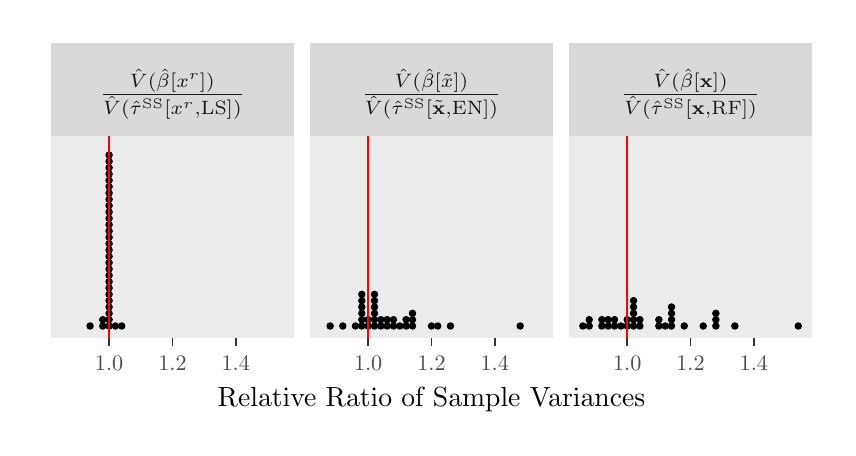
\begin{tikzpicture}[x=1pt,y=1pt]
\definecolor{fillColor}{RGB}{255,255,255}
\path[use as bounding box,fill=fillColor,fill opacity=0.00] (0,0) rectangle (289.08,144.54);
\begin{scope}
\path[clip] (  0.00,  0.00) rectangle (289.08,144.54);
\definecolor{drawColor}{RGB}{255,255,255}
\definecolor{fillColor}{RGB}{255,255,255}

\path[draw=drawColor,line width= 0.6pt,line join=round,line cap=round,fill=fillColor] (  0.00,  0.00) rectangle (289.08,144.54);
\end{scope}
\begin{scope}
\path[clip] (  8.25, 32.28) rectangle ( 96.36,105.24);
\definecolor{fillColor}{gray}{0.92}

\path[fill=fillColor] (  8.25, 32.28) rectangle ( 96.36,105.24);
\definecolor{drawColor}{RGB}{0,0,0}
\definecolor{fillColor}{RGB}{0,0,0}

\path[draw=drawColor,line width= 0.4pt,line join=round,fill=fillColor] ( 22.55, 36.74) circle (  1.14);

\path[draw=drawColor,line width= 0.4pt,line join=round,fill=fillColor] ( 27.13, 36.74) circle (  1.14);

\path[draw=drawColor,line width= 0.4pt,line join=round,fill=fillColor] ( 27.13, 39.02) circle (  1.14);

\path[draw=drawColor,line width= 0.4pt,line join=round,fill=fillColor] ( 29.42, 36.74) circle (  1.14);

\path[draw=drawColor,line width= 0.4pt,line join=round,fill=fillColor] ( 29.42, 39.02) circle (  1.14);

\path[draw=drawColor,line width= 0.4pt,line join=round,fill=fillColor] ( 29.42, 41.31) circle (  1.14);

\path[draw=drawColor,line width= 0.4pt,line join=round,fill=fillColor] ( 29.42, 43.60) circle (  1.14);

\path[draw=drawColor,line width= 0.4pt,line join=round,fill=fillColor] ( 29.42, 45.89) circle (  1.14);

\path[draw=drawColor,line width= 0.4pt,line join=round,fill=fillColor] ( 29.42, 48.18) circle (  1.14);

\path[draw=drawColor,line width= 0.4pt,line join=round,fill=fillColor] ( 29.42, 50.47) circle (  1.14);

\path[draw=drawColor,line width= 0.4pt,line join=round,fill=fillColor] ( 29.42, 52.76) circle (  1.14);

\path[draw=drawColor,line width= 0.4pt,line join=round,fill=fillColor] ( 29.42, 55.04) circle (  1.14);

\path[draw=drawColor,line width= 0.4pt,line join=round,fill=fillColor] ( 29.42, 57.33) circle (  1.14);

\path[draw=drawColor,line width= 0.4pt,line join=round,fill=fillColor] ( 29.42, 59.62) circle (  1.14);

\path[draw=drawColor,line width= 0.4pt,line join=round,fill=fillColor] ( 29.42, 61.91) circle (  1.14);

\path[draw=drawColor,line width= 0.4pt,line join=round,fill=fillColor] ( 29.42, 64.20) circle (  1.14);

\path[draw=drawColor,line width= 0.4pt,line join=round,fill=fillColor] ( 29.42, 66.49) circle (  1.14);

\path[draw=drawColor,line width= 0.4pt,line join=round,fill=fillColor] ( 29.42, 68.78) circle (  1.14);

\path[draw=drawColor,line width= 0.4pt,line join=round,fill=fillColor] ( 29.42, 71.06) circle (  1.14);

\path[draw=drawColor,line width= 0.4pt,line join=round,fill=fillColor] ( 29.42, 73.35) circle (  1.14);

\path[draw=drawColor,line width= 0.4pt,line join=round,fill=fillColor] ( 29.42, 75.64) circle (  1.14);

\path[draw=drawColor,line width= 0.4pt,line join=round,fill=fillColor] ( 29.42, 77.93) circle (  1.14);

\path[draw=drawColor,line width= 0.4pt,line join=round,fill=fillColor] ( 29.42, 80.22) circle (  1.14);

\path[draw=drawColor,line width= 0.4pt,line join=round,fill=fillColor] ( 29.42, 82.51) circle (  1.14);

\path[draw=drawColor,line width= 0.4pt,line join=round,fill=fillColor] ( 29.42, 84.80) circle (  1.14);

\path[draw=drawColor,line width= 0.4pt,line join=round,fill=fillColor] ( 29.42, 87.08) circle (  1.14);

\path[draw=drawColor,line width= 0.4pt,line join=round,fill=fillColor] ( 29.42, 89.37) circle (  1.14);

\path[draw=drawColor,line width= 0.4pt,line join=round,fill=fillColor] ( 29.42, 91.66) circle (  1.14);

\path[draw=drawColor,line width= 0.4pt,line join=round,fill=fillColor] ( 29.42, 93.95) circle (  1.14);

\path[draw=drawColor,line width= 0.4pt,line join=round,fill=fillColor] ( 29.42, 96.24) circle (  1.14);

\path[draw=drawColor,line width= 0.4pt,line join=round,fill=fillColor] ( 29.42, 98.53) circle (  1.14);

\path[draw=drawColor,line width= 0.4pt,line join=round,fill=fillColor] ( 31.71, 36.74) circle (  1.14);

\path[draw=drawColor,line width= 0.4pt,line join=round,fill=fillColor] ( 34.00, 36.74) circle (  1.14);
\definecolor{drawColor}{RGB}{255,0,0}

\path[draw=drawColor,line width= 0.6pt,line join=round] ( 29.42, 32.28) -- ( 29.42,105.24);
\end{scope}
\begin{scope}
\path[clip] (101.86, 32.28) rectangle (189.97,105.24);
\definecolor{fillColor}{gray}{0.92}

\path[fill=fillColor] (101.86, 32.28) rectangle (189.97,105.24);
\definecolor{drawColor}{RGB}{0,0,0}
\definecolor{fillColor}{RGB}{0,0,0}

\path[draw=drawColor,line width= 0.4pt,line join=round,fill=fillColor] (109.30, 36.74) circle (  1.14);

\path[draw=drawColor,line width= 0.4pt,line join=round,fill=fillColor] (113.88, 36.74) circle (  1.14);

\path[draw=drawColor,line width= 0.4pt,line join=round,fill=fillColor] (118.45, 36.74) circle (  1.14);

\path[draw=drawColor,line width= 0.4pt,line join=round,fill=fillColor] (120.74, 36.74) circle (  1.14);

\path[draw=drawColor,line width= 0.4pt,line join=round,fill=fillColor] (120.74, 39.02) circle (  1.14);

\path[draw=drawColor,line width= 0.4pt,line join=round,fill=fillColor] (120.74, 41.31) circle (  1.14);

\path[draw=drawColor,line width= 0.4pt,line join=round,fill=fillColor] (120.74, 43.60) circle (  1.14);

\path[draw=drawColor,line width= 0.4pt,line join=round,fill=fillColor] (120.74, 45.89) circle (  1.14);

\path[draw=drawColor,line width= 0.4pt,line join=round,fill=fillColor] (120.74, 48.18) circle (  1.14);

\path[draw=drawColor,line width= 0.4pt,line join=round,fill=fillColor] (123.03, 36.74) circle (  1.14);

\path[draw=drawColor,line width= 0.4pt,line join=round,fill=fillColor] (123.03, 39.02) circle (  1.14);

\path[draw=drawColor,line width= 0.4pt,line join=round,fill=fillColor] (125.32, 36.74) circle (  1.14);

\path[draw=drawColor,line width= 0.4pt,line join=round,fill=fillColor] (125.32, 39.02) circle (  1.14);

\path[draw=drawColor,line width= 0.4pt,line join=round,fill=fillColor] (125.32, 41.31) circle (  1.14);

\path[draw=drawColor,line width= 0.4pt,line join=round,fill=fillColor] (125.32, 43.60) circle (  1.14);

\path[draw=drawColor,line width= 0.4pt,line join=round,fill=fillColor] (125.32, 45.89) circle (  1.14);

\path[draw=drawColor,line width= 0.4pt,line join=round,fill=fillColor] (125.32, 48.18) circle (  1.14);

\path[draw=drawColor,line width= 0.4pt,line join=round,fill=fillColor] (127.61, 36.74) circle (  1.14);

\path[draw=drawColor,line width= 0.4pt,line join=round,fill=fillColor] (127.61, 39.02) circle (  1.14);

\path[draw=drawColor,line width= 0.4pt,line join=round,fill=fillColor] (129.90, 36.74) circle (  1.14);

\path[draw=drawColor,line width= 0.4pt,line join=round,fill=fillColor] (129.90, 39.02) circle (  1.14);

\path[draw=drawColor,line width= 0.4pt,line join=round,fill=fillColor] (132.18, 36.74) circle (  1.14);

\path[draw=drawColor,line width= 0.4pt,line join=round,fill=fillColor] (132.18, 39.02) circle (  1.14);

\path[draw=drawColor,line width= 0.4pt,line join=round,fill=fillColor] (134.47, 36.74) circle (  1.14);

\path[draw=drawColor,line width= 0.4pt,line join=round,fill=fillColor] (136.76, 36.74) circle (  1.14);

\path[draw=drawColor,line width= 0.4pt,line join=round,fill=fillColor] (136.76, 39.02) circle (  1.14);

\path[draw=drawColor,line width= 0.4pt,line join=round,fill=fillColor] (139.05, 36.74) circle (  1.14);

\path[draw=drawColor,line width= 0.4pt,line join=round,fill=fillColor] (139.05, 39.02) circle (  1.14);

\path[draw=drawColor,line width= 0.4pt,line join=round,fill=fillColor] (139.05, 41.31) circle (  1.14);

\path[draw=drawColor,line width= 0.4pt,line join=round,fill=fillColor] (145.92, 36.74) circle (  1.14);

\path[draw=drawColor,line width= 0.4pt,line join=round,fill=fillColor] (148.20, 36.74) circle (  1.14);

\path[draw=drawColor,line width= 0.4pt,line join=round,fill=fillColor] (152.78, 36.74) circle (  1.14);

\path[draw=drawColor,line width= 0.4pt,line join=round,fill=fillColor] (177.96, 36.74) circle (  1.14);
\definecolor{drawColor}{RGB}{255,0,0}

\path[draw=drawColor,line width= 0.6pt,line join=round] (123.03, 32.28) -- (123.03,105.24);
\end{scope}
\begin{scope}
\path[clip] (195.47, 32.28) rectangle (283.58,105.24);
\definecolor{fillColor}{gray}{0.92}

\path[fill=fillColor] (195.47, 32.28) rectangle (283.58,105.24);
\definecolor{drawColor}{RGB}{0,0,0}
\definecolor{fillColor}{RGB}{0,0,0}

\path[draw=drawColor,line width= 0.4pt,line join=round,fill=fillColor] (200.62, 36.74) circle (  1.14);

\path[draw=drawColor,line width= 0.4pt,line join=round,fill=fillColor] (202.91, 36.74) circle (  1.14);

\path[draw=drawColor,line width= 0.4pt,line join=round,fill=fillColor] (202.91, 39.02) circle (  1.14);

\path[draw=drawColor,line width= 0.4pt,line join=round,fill=fillColor] (207.48, 36.74) circle (  1.14);

\path[draw=drawColor,line width= 0.4pt,line join=round,fill=fillColor] (207.48, 39.02) circle (  1.14);

\path[draw=drawColor,line width= 0.4pt,line join=round,fill=fillColor] (209.77, 36.74) circle (  1.14);

\path[draw=drawColor,line width= 0.4pt,line join=round,fill=fillColor] (209.77, 39.02) circle (  1.14);

\path[draw=drawColor,line width= 0.4pt,line join=round,fill=fillColor] (212.06, 36.74) circle (  1.14);

\path[draw=drawColor,line width= 0.4pt,line join=round,fill=fillColor] (212.06, 39.02) circle (  1.14);

\path[draw=drawColor,line width= 0.4pt,line join=round,fill=fillColor] (214.35, 36.74) circle (  1.14);

\path[draw=drawColor,line width= 0.4pt,line join=round,fill=fillColor] (216.64, 36.74) circle (  1.14);

\path[draw=drawColor,line width= 0.4pt,line join=round,fill=fillColor] (216.64, 39.02) circle (  1.14);

\path[draw=drawColor,line width= 0.4pt,line join=round,fill=fillColor] (218.93, 36.74) circle (  1.14);

\path[draw=drawColor,line width= 0.4pt,line join=round,fill=fillColor] (218.93, 39.02) circle (  1.14);

\path[draw=drawColor,line width= 0.4pt,line join=round,fill=fillColor] (218.93, 41.31) circle (  1.14);

\path[draw=drawColor,line width= 0.4pt,line join=round,fill=fillColor] (218.93, 43.60) circle (  1.14);

\path[draw=drawColor,line width= 0.4pt,line join=round,fill=fillColor] (218.93, 45.89) circle (  1.14);

\path[draw=drawColor,line width= 0.4pt,line join=round,fill=fillColor] (221.22, 36.74) circle (  1.14);

\path[draw=drawColor,line width= 0.4pt,line join=round,fill=fillColor] (221.22, 39.02) circle (  1.14);

\path[draw=drawColor,line width= 0.4pt,line join=round,fill=fillColor] (228.08, 36.74) circle (  1.14);

\path[draw=drawColor,line width= 0.4pt,line join=round,fill=fillColor] (228.08, 39.02) circle (  1.14);

\path[draw=drawColor,line width= 0.4pt,line join=round,fill=fillColor] (230.37, 36.74) circle (  1.14);

\path[draw=drawColor,line width= 0.4pt,line join=round,fill=fillColor] (232.66, 36.74) circle (  1.14);

\path[draw=drawColor,line width= 0.4pt,line join=round,fill=fillColor] (232.66, 39.02) circle (  1.14);

\path[draw=drawColor,line width= 0.4pt,line join=round,fill=fillColor] (232.66, 41.31) circle (  1.14);

\path[draw=drawColor,line width= 0.4pt,line join=round,fill=fillColor] (232.66, 43.60) circle (  1.14);

\path[draw=drawColor,line width= 0.4pt,line join=round,fill=fillColor] (237.24, 36.74) circle (  1.14);

\path[draw=drawColor,line width= 0.4pt,line join=round,fill=fillColor] (244.10, 36.74) circle (  1.14);

\path[draw=drawColor,line width= 0.4pt,line join=round,fill=fillColor] (248.68, 36.74) circle (  1.14);

\path[draw=drawColor,line width= 0.4pt,line join=round,fill=fillColor] (248.68, 39.02) circle (  1.14);

\path[draw=drawColor,line width= 0.4pt,line join=round,fill=fillColor] (248.68, 41.31) circle (  1.14);

\path[draw=drawColor,line width= 0.4pt,line join=round,fill=fillColor] (255.54, 36.74) circle (  1.14);

\path[draw=drawColor,line width= 0.4pt,line join=round,fill=fillColor] (278.43, 36.74) circle (  1.14);
\definecolor{drawColor}{RGB}{255,0,0}

\path[draw=drawColor,line width= 0.6pt,line join=round] (216.64, 32.28) -- (216.64,105.24);
\end{scope}
\begin{scope}
\path[clip] (  8.25,105.24) rectangle ( 96.36,139.04);
\definecolor{fillColor}{gray}{0.85}

\path[fill=fillColor] (  8.25,105.24) rectangle ( 96.36,139.04);
\definecolor{drawColor}{gray}{0.10}

\node[text=drawColor,anchor=base,inner sep=0pt, outer sep=0pt, scale=  1.00] at ( 52.31,125.21) {};

\node[text=drawColor,anchor=base,inner sep=0pt, outer sep=0pt, scale=  1.00] at ( 52.31,118.01) {$\frac{\hat{\mathbb{V}}(\hat{\beta}[x^r])}{\hat{\mathbb{V}}(\hat{\tau}^{\mathrm{SS}}[x^r,\mathrm{LS}])}$};

\node[text=drawColor,anchor=base,inner sep=0pt, outer sep=0pt, scale=  1.00] at ( 52.31,110.81) {};
\end{scope}
\begin{scope}
\path[clip] (101.86,105.24) rectangle (189.97,139.04);
\definecolor{fillColor}{gray}{0.85}

\path[fill=fillColor] (101.86,105.24) rectangle (189.97,139.04);
\definecolor{drawColor}{gray}{0.10}

\node[text=drawColor,anchor=base,inner sep=0pt, outer sep=0pt, scale=  1.00] at (145.92,125.21) {};

\node[text=drawColor,anchor=base,inner sep=0pt, outer sep=0pt, scale=  1.00] at (145.92,118.01) {$\frac{\hat{\mathbb{V}}(\hat{\beta}[\tilde{x}])}{\hat{\mathbb{V}}(\hat{\tau}^{\mathrm{SS}}[\tilde{\mathbf{x}},\mathrm{EN}])}$};

\node[text=drawColor,anchor=base,inner sep=0pt, outer sep=0pt, scale=  1.00] at (145.92,110.81) {};
\end{scope}
\begin{scope}
\path[clip] (195.47,105.24) rectangle (283.58,139.04);
\definecolor{fillColor}{gray}{0.85}

\path[fill=fillColor] (195.47,105.24) rectangle (283.58,139.04);
\definecolor{drawColor}{gray}{0.10}

\node[text=drawColor,anchor=base,inner sep=0pt, outer sep=0pt, scale=  1.00] at (239.52,125.21) {};

\node[text=drawColor,anchor=base,inner sep=0pt, outer sep=0pt, scale=  1.00] at (239.52,118.01) {$\frac{\hat{\mathbb{V}}(\hat{\beta}[\mathbf{x}])}{\hat{\mathbb{V}}(\hat{\tau}^{\mathrm{SS}}[\mathbf{x},\mathrm{RF}])}$};

\node[text=drawColor,anchor=base,inner sep=0pt, outer sep=0pt, scale=  1.00] at (239.52,110.81) {};
\end{scope}
\begin{scope}
\path[clip] (  0.00,  0.00) rectangle (289.08,144.54);
\definecolor{drawColor}{gray}{0.20}

\path[draw=drawColor,line width= 0.6pt,line join=round] ( 29.42, 29.53) --
	( 29.42, 32.28);

\path[draw=drawColor,line width= 0.6pt,line join=round] ( 52.31, 29.53) --
	( 52.31, 32.28);

\path[draw=drawColor,line width= 0.6pt,line join=round] ( 75.19, 29.53) --
	( 75.19, 32.28);
\end{scope}
\begin{scope}
\path[clip] (  0.00,  0.00) rectangle (289.08,144.54);
\definecolor{drawColor}{gray}{0.30}

\node[text=drawColor,anchor=base,inner sep=0pt, outer sep=0pt, scale=  0.80] at ( 29.42, 20.71) {1.0};

\node[text=drawColor,anchor=base,inner sep=0pt, outer sep=0pt, scale=  0.80] at ( 52.31, 20.71) {1.2};

\node[text=drawColor,anchor=base,inner sep=0pt, outer sep=0pt, scale=  0.80] at ( 75.19, 20.71) {1.4};
\end{scope}
\begin{scope}
\path[clip] (  0.00,  0.00) rectangle (289.08,144.54);
\definecolor{drawColor}{gray}{0.20}

\path[draw=drawColor,line width= 0.6pt,line join=round] (123.03, 29.53) --
	(123.03, 32.28);

\path[draw=drawColor,line width= 0.6pt,line join=round] (145.92, 29.53) --
	(145.92, 32.28);

\path[draw=drawColor,line width= 0.6pt,line join=round] (168.80, 29.53) --
	(168.80, 32.28);
\end{scope}
\begin{scope}
\path[clip] (  0.00,  0.00) rectangle (289.08,144.54);
\definecolor{drawColor}{gray}{0.30}

\node[text=drawColor,anchor=base,inner sep=0pt, outer sep=0pt, scale=  0.80] at (123.03, 20.71) {1.0};

\node[text=drawColor,anchor=base,inner sep=0pt, outer sep=0pt, scale=  0.80] at (145.92, 20.71) {1.2};

\node[text=drawColor,anchor=base,inner sep=0pt, outer sep=0pt, scale=  0.80] at (168.80, 20.71) {1.4};
\end{scope}
\begin{scope}
\path[clip] (  0.00,  0.00) rectangle (289.08,144.54);
\definecolor{drawColor}{gray}{0.20}

\path[draw=drawColor,line width= 0.6pt,line join=round] (216.64, 29.53) --
	(216.64, 32.28);

\path[draw=drawColor,line width= 0.6pt,line join=round] (239.53, 29.53) --
	(239.53, 32.28);

\path[draw=drawColor,line width= 0.6pt,line join=round] (262.41, 29.53) --
	(262.41, 32.28);
\end{scope}
\begin{scope}
\path[clip] (  0.00,  0.00) rectangle (289.08,144.54);
\definecolor{drawColor}{gray}{0.30}

\node[text=drawColor,anchor=base,inner sep=0pt, outer sep=0pt, scale=  0.80] at (216.64, 20.71) {1.0};

\node[text=drawColor,anchor=base,inner sep=0pt, outer sep=0pt, scale=  0.80] at (239.53, 20.71) {1.2};

\node[text=drawColor,anchor=base,inner sep=0pt, outer sep=0pt, scale=  0.80] at (262.41, 20.71) {1.4};
\end{scope}
\begin{scope}
\path[clip] (  0.00,  0.00) rectangle (289.08,144.54);
\definecolor{drawColor}{RGB}{0,0,0}

\node[text=drawColor,anchor=base,inner sep=0pt, outer sep=0pt, scale=  1.00] at (145.91,  7.83) {Relative Ratio of Sample Variances};
\end{scope}
\end{tikzpicture}
